\documentclass{article}
\usepackage{tabularx}
\usepackage{pdflscape}
\usepackage{graphicx}

\graphicspath{ {./} }

\newcolumntype{s}{>{\hsize=0.2\hsize}>{\centering}X}
\newcolumntype{m}{>{\hsize=1.0\hsize}>{\centering}X}
\newcolumntype{b}{>{\hsize=1.8\hsize}>{\centering}X}

% Enter the name of the subject
\newcommand{\assignmentname}{Assignment 4: Testing}
% Your names
\newcommand{\studentA}{Evelien Daems}
\newcommand{\studentB}{Lars Van Roy}

\title{\textmd{\textbf{Software Engineering}}\\\normalsize\vspace{0.1in}\Large{\assignmentname}\\\vspace{0.1in}\small{\textit{3 Ba INF \  2018-2019}}}
\author{\studentA \\ \studentB}

\begin{document}
\maketitle
\noindent
\textbf{Calculate() function analysis} \newline
\newline
\maketitle
\noindent
\underline{Control Flow Graph}\newline
\newline
Een control flow graph is een visuele weergave van een programma waarmee alle mogelijke paden doorheen een programma kunnen gegenereerd worden. Elke binaire node (een node waar twee pijlen uitkomen) komt overheen met een conditie in het programma. Elke mogelijke sequentie van nodes dat eindigt in een eindstaat is een mogelijk pad door het programma, het is echter niet gegarandeerd dat dit pad ook bestaat. Sommige condities kunnen enkel slagen indien andere condities ook slagen en of slagen sowieso x aantal keren. Het is dus niet omdat de sequentie bestaat in de control flow graph dat het ook een mogelijk pad is. Voor de flow graph van de calculate() functie zie appendix A. \\
\newline
\maketitle
\noindent
\underline{Cyclomatic Complexity}\newline
\newline
De cyclomatic complexity kan berekend worden door het aantal edges - het aantal nodes te beschouwen + 2 of het aantal binaire conditie nodes + 1. Beide geven ons in dit geval 10. Deze waarde symboliseert een bovengrens voor het aantal mogelijke onafhankelijke paden door de flowgraph. \\
aantal edges - aantal nodes + 2 = 29 - 21 + 2 = 10 \\
aantal binarie condities + 1 = 9 + 1 = 10 \\

\newpage
\maketitle
\noindent
\underline{independent paths}\newline
\newline
Wanneer we beginnend van het kortst mogelijke pad verdergaan door steeds een nieuw onafhankelijke pad te nemen krijgen we een mogelijkheid om de verschillende paden voor te stellen. Een nieuw pad wordt onafhankelijk genoemd van de voorgaande paden als er in het nieuwe pad een node voorkomt die nog niet voorkwam in de voorgaande paden. Wanneer we dit doen bekomen we de volgende paden. \\

\begin{table}[h]
	\centering
	\begin{tabularx}{\linewidth}{| s | b |}
		\hline
		index & pad \tabularnewline
		\hline
		0 & {1, 2, 6, 7, 21} \tabularnewline
		\hline
		1 & {1, 2, 6, 7, 8, 9, 10, 7, 21} \tabularnewline
		\hline
		2 & {1, 2, 3, 2, 6, 7, 8, 9, 10, 7, 21} \tabularnewline
		\hline
		3 & {1, 2, 3, 4, 5, 2, 6, 7, 21} \tabularnewline
		\hline
		4 & {1, 2, 3, 4, 5, 2, 6, 7, 8, 9, 10, 11, 12, 10, 7, 21} \tabularnewline
		\hline
		5 & {1, 2, 3, 4, 5, 2, 6, 7, 8, 9, 10, 11, 12, 13, 14, 12, 10, 7, 21} \tabularnewline
		\hline
		6 & {1, 2, 3, 4, 5, 2, 6, 7, 8, 9, 10, 11, 12, 13, 14, 15, 12, 10, 7, 21} \tabularnewline
		\hline
		7 & {1, 2, 3, 4, 5, 2, 6, 7, 8, 9, 10, 11, 12, 13, 14, 15, 16, 17, 12, 10, 7, 21} \tabularnewline
		\hline
		8 & {1, 2, 3, 4, 5, 2, 6, 7, 8, 9, 10, 11, 12, 13, 14, 15, 16, 17, 18, 12, 10, 7, 21} \tabularnewline
		\hline
		9 & {1, 2, 3, 4, 5, 2, 6, 7, 8, 9, 10, 11, 12, 13, 14, 15, 16, 17, 18, 19, 20, 12, 10, 12, 10, 7, 10, 12, 10, 7, 21} \tabularnewline
		\hline
	\end{tabularx}
	\caption{alle mogelijke paden}
\end{table}

\newpage
\maketitle
\noindent
\underline{test cases}\newline
\newline
Bij nadere observatie van deze paden zien we dat het merendeel hiervan niet bereikbaar is. sommige condities kunnen niet falen zonder dat andere in het programma ook falen en omgekeerd. Uiteindelijk blijven volgende 4 paden over met bijhorende input en output. Hierbij zijn triviale inputvelden, of m.a.w. inputvelden waarvoor de waarde niet relevant is om het gewenste pad te bekomen, weggelaten. Een volledig overzicht van alle paden en welke paden nu uiteindelijk een bestaand pad door de functie hadden zijn weergegeven in appendix B.\\

\begin{table}[h]
	\centering
	\begin{tabularx}{\linewidth}{| s | b | m |}
		\hline
		index & input & output \tabularnewline
		\hline
		1 & m\_db\.m\_tidlist = \{\} & \{\{\}, \{\}\} \tabularnewline
		\hline
		2 & m\_db\.m\_tidlist = \{0:\{0\}\}; \newline min\_sup = 2; & \{\{\}, \{\}\} \tabularnewline
		\hline
		4 & m\_db\.m\_tidlist = \{0:\{0\}\}; \newline min\_sup = 1; & \{\{[0]\}, \{\}\} \tabularnewline
		\hline
		9 & m\_db\.m\_tidlist = \{0:\{1,2\}, 1:\{1\}\}; \newline min\_sup = 1; & \{\{[0], [1]\}, \{[0, 1]\}, \{\}\} \tabularnewline
		\hline
	\end{tabularx}
	\caption{test cases}
\end{table}

\newpage
\maketitle
\noindent
\textbf{JUnit testing}\newline
\newline

\maketitle
\noindent
\underline{unit tests}\newline
\newline
Unit tests zijn testen waarbij kleine stukjes code apart worden getest zonder afhankelijkheden etc. Door dit te doen kunnen we specifiek zoeken naar fouten in de implementatie binnen een unit. Voor elke unit worden er meerdere testcases doorlopen. Voor het core.Clients packet onderscheiden we 6 verschillende units, zijnde: Address, Client, Mailing\_Preferences, RegisteredClient, UnregisteredClient en Clients. \newline
\newline
Voor elk van deze units schrijven we voor elke methode één of meerdere testen waarbij we de verwachte output vergelijken met de eigenlijke output.\newline
\newline
Dit lukt voor 3 van de 6 units maar bij de 3 andere zijn er assertions die foutieve returns opvangen. \newline
\newline
In de unit Client faalt de methode getRegisteredClient(string, string) om de gewenste return te geven. Deze zou, indien er bestaande data wordt opgegeven, een referentie moeten geven naar het gerefereerde Client object maar dit doet hij niet, hij returned null onafhankelijk van de gegeven input.\newline
\newline
In de unit Mailing\_preferences faalt de functie third\_party() in sommige gevallen. Wanneer de constructor input gelijk is aan (true, true, true) is er geen probleem maar wanneer de constructor input gelijk is aan (true, true, false) geeft de funtie third\_party() plots ook true terug. Wanneer de constructor input krijgt gelijk aan (false, false, false) werkt alles wel weer normaal. \newline
\newline
Ten slotte heeft de unit RegisteredClient nog een probleem in de functie checkPassword(string). Deze functie zou true moeten return indien het correcte wachtwoord wordt meegegeven als string maar dit is niet het geval.

\newpage
\maketitle
\noindent
\underline{integration tests}\newline
\newline
Integration tests zijn testen waarbij meerdere units samen getest worden. Door dit te doen kunnen we zoeken naar fouten in afhankelijkheden in units. Indien alle unittesten slagen weten we dat er niet zozeer problemen zijn in de units op zich maar dat er fouten zijn in het gebruik van de methoden van andere units.\newline
\newline
Deze test bestaat in essentie uit hetzelfde als de unit tests. We maken opnieuw gebruik van verschillende methodes maar in plaats van enkel methodes van 1 unit te beschouwen beschouwen we meerdere methoden uit meerdere units en het effect dat ze op andere methoden kunnen hebben. \newline
\newline
In de beschouwde integration test worden de calls naar methoden uit core.Clients in het pakket Core onderzocht. Deze methoden worden voor zover de test reikt goed gebruikt en de teruggegeven waarden komen steeds overeen met de verwachte output.\newline
\newline
\maketitle
\noindent
\underline{synopsis voor testen}\newline
\newline
Testen zijn nooit volledig, er zijn steeds methoden die voor sommige situaties wel slagen en voor andere niet. Het is zeer moeilijk om af te wegen wanneer er genoeg testen geschreven zijn. De bedoeling is niet dat het uren duurt om deze testen uit te voeren voor methodes die geen vitale belangen hebben in het verloop van het programma en al evenmin dat er maar een paar testen worden geschreven voor functionaliteiten waarop het hele programma gebaseerd is. Het is dus belangrijk om hier een afweging in te maken.\newline
\newline
Ook al zijn niet altijd alle situaties beschouwd, door een percentage van alle mogelijke situaties te beschouwen en hierop extensief te testen beperken we wel het risico op fouten. Er is namelijk een deel van de situaties die zich kunnen voordoen die getest zijn en waarin niets meer zou mogen vastlopen. \newline
\newline
Ten slotte is het ook belangrijk om zowel unit tests als integration tests te gebruiken. Unit tests zijn zeer handig om fouten binnen units op te zoeken maar deze zijn niet toereikend over het gehele systeem. Fouten die ontstaan door combinaties van units zijn veel voorkomend en moeilijker te vinden dan fouten in units zelf dus is het ook belangrijk om integration tests te schrijven.

\newpage
\maketitle
\noindent
\textbf{Design by contract} \newline
\newline

\maketitle
\noindent
In het algemeen vereisen we bij elke functionaliteiten dat er geen operatie kan worden verricht op null objecten en dat de teruggegeven waarden eveneens geen null object kunnen bevatten.\newline
\newline

\noindent
\underline{Class Catalog}\newline
\textit{@requires(\{"item!=null", "\$this.findMatch(item) == null"\})}\newline
\textit{@ensures("\$old(\$this.getNumberOfItems())+1==\$this.getNumberOfItems()")}\newline
\textit{public void addItem(Item item) \{...\}}\newline
Voor het toevoegen van een item aan de catalogus wordt er door de klant evreist dat alle items uniek moeten zijn op basis van hun naam, beschrijving en prijs. Dit moet eerst worden gecontroleerd voordat we het item gaan toevoegen aan de catalogus. Nadien moet men verifi\"{e}ren of het item met succes is toegevoegd aan de catalogus. Anders zou de gebruiker er vanuitgaan dat dit item is toegevoegd en dit item gaan oproepen in een ander deel van het systeem om dan pas te ontdekken dat dit item nooit toegevoegd is geweest.\\

\noindent
\textit{@requires(\{"item!=null"\})}\newline
\textit{public Item findMatch(Item item)\{...\}}\newline
Een eigen geschreven functionaliteit om aan de specificatie te voldoen waarin beschreven staat dat een Item uniek moet zijn in de zin van een unieke naam, beschrijving en prijs in de catalogus. Hier is het wel toegestaan om een return waarde te hebben van null aangezien dit betekent dat geen enkel item werd gevonden dat overeenkwam met de input. \\

\newpage

\underline{Class Cart}\newline
\textit{@requires(\{"quantity$>$=0", "item!=null"\})}\newline
\textit{@ensures("\$old(\$this.contents().get(item))+quantity==\$this.contents().get(item)")}\newline
\textit{public void addItem(Item item, int quantity)\{...\}}\newline
Bij het toevoegen van een item aan een Cart object is het belangrijk dat het item een bestaand en geïnstantieerd object is. Want voor de gebruiker heeft het geen zin dat er een ijdel object wordt toegevoegd aan het winkelwagentje. Dit zou eveneens problemen kunnen geven bij verdere bewerkingen op Cart en dus onderweg voor errors kunnen zorgen. De vereiste dat een posititef aantal moet worden toegevoegd, is natuurlijk triviaal want het is onrealistisch dat een gebruiker een negatief aantal items in zijn of haar winkelwagen wil.\newline
Na het toevoegen van een item moet er gegarandeerd worden dat er niets is mis gegaan tijdens het toevoegen. We zullen dus eisen dat de oude winkelwagen is geupdate met het gevraagde item en bijhorende hoeveelheid. \\

\noindent
\textit{@requires(\{"\$old(\$this.contents().containsKey(item)==true", "item!=null", "quantity$>$=0"\})} \newline
\textit{@ensures("\$this.contents().get(item)==\$old(\$this.contents().get(item))-quantity")} \newline
\textit{public void removeItem(Item item, int quantity) \{...\}} \newline
Voor een item kan verwijderd worden is het belangrijk te controleren of dit ook effectief aanwezig is in de content van het Cart object. Quantity moet een positief getal zijn om een correct verloop van de removeItem() functionaliteit te garanderen. Indien een gebruiker toevallig een negatief getal zou toekennen aan de parameter dan voldoet het resultaat van de functie niet meer aan de verwachtingen die men heeft bij het uitvoeren. Dan zou het verwijderen resulteren in het toevoegen van items. Idem aan de functie addItem() eisen we de garantie dat een item effecief verminderd is in hoeveelheid met aantal quantity. \\

\noindent
\textit{@requires(\{"\$this.contents()!=null"\})}\newline
\textit{@ensures(\{"\$result$>$=0", "\$result!=null"\})}\newline
\textit{private float getCostFloat()\{...\}}\newline
Deze functie hebben we zelf toegevoegd om de totale waarde van de winkelwagen in float notatie te berekenen. De contents van het object moet geïnitialiseerd zijn om de kost te kunnen berekenen en het resultaat kan niet negatief zijn. Indien dit wel het geval is zou de webshop de klant gaan betalen om producten te kopen, wat helemaal niet de bedoeling is. Het resultaat moet ook bestaan indien alles goed is verlopen.\\

\noindent
\textit{@ensures(\{"\$result != null, \$result.length()!=0"\})}\newline
\textit{public String getCost() \{...\}}\newline
Dit is de functionalieit die de totale prijs van de winkelwagen zal teruggeven in tekst formaat. Als gebruiker verwachten we een geldige return waarde die nooit leeg kan zijn als alles goed is verlopen.\\

\newpage

\noindent
\underline{Class Category}\newline
\textit{@ensures("\$this.getCategories().length()==10")}\newline
\textit{public Category()\{...\}}\newline
De Catalog moet verplicht standaard 10 categori\"{e}n bevatten die staan opgesomd in de specificaties van de klant. Dus zorgen voor een postconditie die kijkt of bij het aanmaken van de Catalog de lijst ook effectief bestaat uit deze categori\"{e}n. Het is niet nodig om per categorie te gaan kijken of er wel de juiste in staan want dit zit hardcoded in het programma. Het is enkel nodig om te kijken of de lijst niet leeg is en wat er dus op zou kunnen duiden dat er iets is misgegaan bij het aanmaken van het object.\\

\noindent
\textit{@requires(\{"category.length()!=0", "!\$this.getCategories().contains(category)"\})}\newline
\textit{@ensures(\{"\$this.getCategories().contains(category)==true", "\$old(\$this.getCategories().size())+1==\$this.getCategories().size()"\})}\newline
\textit{public void addCategory(String category)\{...\}}\newline
Voor het toevoegen van een categorie toe te laten, willen we eerst kijken of categorie geen lege string is, want het is onmogelijk om een lege categorie te hebben. Ten tweede moeten alle categori\"{e}n uniek zijn en controleren we of de in te voegen string als geen deel uitmaakt van de categori\"{e}n. \\

\noindent
\underline{Class Item}\newline
\textit{@requires(\{"price > 0"\})}\newline
\textit{public Item(String name, String desc, float price) \{...\}}\newline
De prijs van een item in de catalogus moet een niet-nul positief getal zijn volgens de specificaties.


\newpage
\maketitle
\noindent
\textbf{appendix A}\newline
\newline
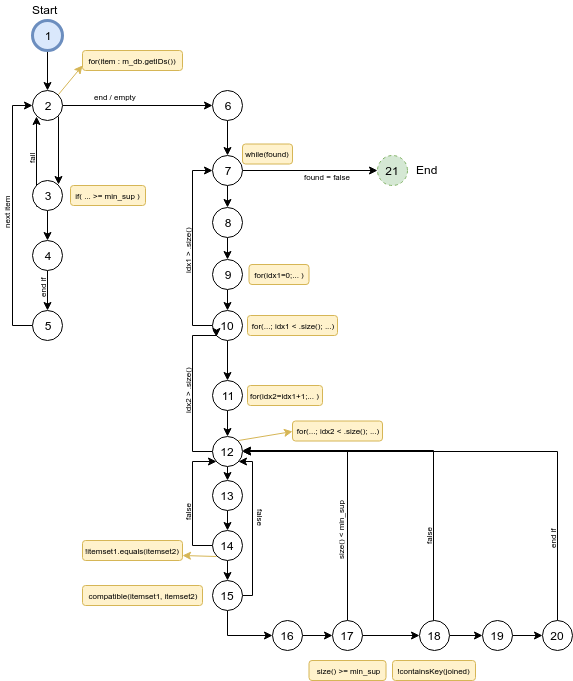
\includegraphics[width=\textwidth]{control_flow_graph}

\newpage
\begin{landscape}
	\maketitle
	\noindent
	\textbf{appendix B}\newline
	\newline
	\begin{table}[h]
		\centering
		\begin{tabularx}{\linewidth}{| >{\hsize=0.3\hsize}>{\centering}X | >{\hsize=1.35\hsize}>{\centering}X | >{\hsize=1.35\hsize}>{\centering}X | >{\hsize=1\hsize}>{\centering}X |}
			\hline
			index & pad & input & output \tabularnewline
			\hline
			0 & {1, 2, 6, 7, 21} & bestaat niet & bestaat niet\tabularnewline
			\hline
			1 & {1, 2, 6, 7, 8, 9, 10, 7, 21} & m\_db\.m\_tidlist = \{\} & \{\{\}, \{\}\} \tabularnewline
			\hline
			2 & {1, 2, 3, 2, 6, 7, 8, 9, 10, 7, 21} & m\_db\.m\_tidlist = \{0:\{0\}\}; \newline min\_sup = 2; & \{\{[0]\}, \{\}\} \tabularnewline
			\hline
			3 & {1, 2, 3, 4, 5, 2, 6, 7, 21} & bestaat niet & bestaat niet \tabularnewline
			\hline
			4 & {1, 2, 3, 4, 5, 2, 6, 7, 8, 9, 10, 11, 12, 10, 7, 21} & m\_db\.m\_tidlist = \{0:\{0\}\}; \newline min\_sup = 1; & \{\{[0]\}, \{\}\} \tabularnewline
			\hline
			5 & {1, 2, 3, 4, 5, 2, 6, 7, 8, 9, 10, 11, 12, 13, 14, 12, 10, 7, 21} & bestaat niet & bestaat niet\tabularnewline
			\hline
			6 & {1, 2, 3, 4, 5, 2, 6, 7, 8, 9, 10, 11, 12, 13, 14, 15, 12, 10, 7, 21} & bestaat niet & bestaat niet \tabularnewline
			\hline
			7 & {1, 2, 3, 4, 5, 2, 6, 7, 8, 9, 10, 11, 12, 13, 14, 15, 16, 17, 12, 10, 7, 21} & bestaat niet & bestaat niet \tabularnewline
			\hline
			8 & {1, 2, 3, 4, 5, 2, 6, 7, 8, 9, 10, 11, 12, 13, 14, 15, 16, 17, 18, 12, 10, 7, 21} & bestaat niet & bestaat niet \tabularnewline
			\hline
			9 & {1, 2, 3, 4, 5, 2, 6, 7, 8, 9, 10, 11, 12, 13, 14, 15, 16, 17, 18, 19, 20, 12, 10, 12, 10, 7, 10, 12, 10, 7, 21} & bestaat niet & bestaat niet \tabularnewline
			\hline
		\end{tabularx}
		\caption{paden + test cases}
	\end{table}
\end{landscape}

\end{document}